\section{Implementation}
In order to evaluate the need for a domain specific programming language we implemented a basic stream cipher, RC4, 
in a variety of different programming languages. Although it is no longer commonly used or secure, RC4 encompasses 
the basic bitwise operations necessary for implementing cryptographic algorithms. We focus on the base functionality 
of each language and ignore most libraries and API functions beyond what is absolutely necessary. In the case of C we 
assume that the same behavior observed is also true for C++.

\subsection{C}
Commonly used for implementing cryptographic algorithms for kernel development, systems libraries, and embedded applications 
where there is no hardware implementation. C provides maximum freedom out of our implementations as the programmer has access 
to the actual memory locations where data is stored. In the hands of a competent and attentive programmer C allows for maximum 
performance and an assurance that certain memory operations have taken place. Such as zeroing memory with \texttt{memset()} used to store a key after 
it has been freed. Bitwise operations and substitution is relatively easy in C even though there is no access to individual bits. The representation of 
Strings as an array of characters also makes it easy to convert them into arrays of bytes. Lastly, the presence of a multitude of different unsigned 
data types and type checking at compile time helps to protect the programmer from easy mistakes. Most errors, such as type issues, in a program are 
also caught at compile time therefore avoiding costly mistakes from appearing in a production environment.

The same flexibility that manual memory management that C provides is also its greatest weakness. The danger of a buffer overflow is significant with 
applications written in C. Commonly used operations such as \texttt{strcpy()}, \texttt{gets()}, and \texttt{strcmp()} do not check the length of 
their inputs therefore leaving any program using them vulnerable to carefully selected inputs which can leak information. For instance calling any 
string comparison method, like \texttt{strcmp()}, which compares two strings character by character will leak the length of said string. A programmer must also be 
careful when determining the size of a piece of data in memory. If using a structure for managing data padding can be inserted between variables and when the 
function \texttt{sizeof()} is called on a pointer it returns the length of a memory address, not the data at that memory address. Compilers and the standard 
library also pose issues. The standard library is used for many basic operations in C but sadly many parts of this library such as the random number generator 
are not cryptographically secure. Most C compilers offer some form of optimization that can introduce inintended or undefined behavior into the resulting 
program. For instance undefined behavior is especially common when using the second and third optimization settings with the Gnu C Compiler. Lastly even though most 
compilers perform type checking and other error detection at compile time, many problems are expressed as warnings that can easily be ignored by the programmer.

\subsection{Lisp}
Among the many dialects of Lisp available we used Common Lisp, primarily due to its popularity as the name would imply. Lisp allows us to represent our plaintext, 
ciphertext, and key as lists of bytes. Which allows for relatively simple bitwise operations even though as with C we have no access to individual bits. The functional
paradigm also lends itself well to how cryptographic algorithms are constructed. With multiple operations occuring one after the other on a stream of data. The primary 
advantage of Lisp is that it is a garbage collected language. Unlike C this means that the language is memory safe. While enforcement of limits on allocated 
regions of memory removes the possibility for things like buffer overflow and misjudging the size of a region in memory it also hides what machine code is actually 
being executed.

\subsection{Python}
While celebrated for its simplicity, accessibility and similarity to pseudocode often used to express cryptographic algorithms in specifications. Our KSA and PRGA 
in Python are virtually identical to the pseudocode used as a basis for all our implementations. Python is not very well suited to the task of implementing 
cryptographic algorithms. Primarily due to its weak type system that does not enforce anything before running a program. In addition to this major flaw occassionally type 
errors never appear as the Python interpreter may perform implicit type conversions at runtime.

\subsection{Java}
As one of the most commonly used programming languages and a prime example of an object oriented paradigm, Java is an obvious choice for our lineup of programming languages.
Syntactically Java is similar to C and in some cases identical for many of the operations that are used in implementing RC4. The biggest difference being that Java manages 
memory for the programmer and that it lacks a data type for an unsigned byte. This first point is more of an advantage than a drawback as manual memory management is the 
source of most of the weaknesses in C. Although it does open the door for uncertaintly about what is actually being executed by the Java Virtual Machine and whether or not 
its memory is securely being freed. The lack of an unsigned byte type in Java means that while one can represent a stream of bytes as an array, one must either use multiple 
API functions such as a \texttt{BitSet} or juggle type casting and bit masking each time an operation on an individual byte is desired. There is also the fact that 
strings are represented as Java objects instead of as a primitive data type so a user is not entirely sure what could be leaked when converting a string into an array of 
bytes.

\subsection{Cryptol}
The strong typing explicitly declared by the programmer preceding each function that was inherited from Haskell puts Cryptol well ahead of its competition in terms of 
type systems. Cryptol operates on sequences of bits and is really the only family of data types used in the language. Even strings and characters are described as just a 
sequence of bits which makes processing the inputs for a algorithm trivial. Unlike any other language that we have examined Cryptol allows access to individual bits in a 
stream and a fully featured assortment of bitwise operations. For instance our permutation of all possible bytes is described by the type \texttt{[256][8]} and an 
infinite sequence of bytes is expressed as \texttt{[inf][8]}. 

As a derivative of Haskell, Cryptol is a functional language and lacks any form of loop structure. Instead the 
programmer must define recurrence relations which complicates implementation when a algorithm's specification describes using \texttt{for} or \texttt{while} loops like in the 
case of RC4. While generating the key stream cryptol poses some difficulties as to avoid hard coding the length of a key or input ciphertext/plaintext one must express then as 
an infinite sequence of bytes. Some infinitely recursive appending of the key to itself becomes necessary in the PRGA function so that an endless keystream can be generated with 
causing Cryptol to output a type mismatch error. Although the type mismatch error can be seen as a benefit at any problems with data length, inputs, conversions, and bitwise operations 
are detected before the code is actual run. Here we see the greatest benefit of Cryptol in its capacity to verify programs through the Z3 SMT solver. Lastly similar to languages 
like Dafny one can declare "properties" that are checked when the program is run in order to prove its correctness.

\section{Evaluation}
Here we compare our implementations of RC4 in terms of performance, lines of code, and a qualitative analysis. For performance we measure latency and throughput for 
each implementation with the exception of Cryptol as we have not yet found an effective way to benchmark its performance. As for lines of code we count only the lines used to implement the basic functionality of the RC4 algorithm. So for C we have $50$ lines, Java has $43$, Lisp has $45$, Python with $28$, and Cryptol with $32$.

\subsection{Performance}

We evaluated the performance of our implementations for both latency and throughput. In order to measure this we encrypted Mark Antony's 
monologue from Act $3$ Scene $2$ of Shakespeare's play \emph{Julius Caesar} using a relatively short 12 character key. We used Python version 2.7, OpenJDK 8, GNU Clisp 2.49, SBCL 1.3.1, and GCC 5.4. Due to the large variability between the behavior of Common Lisp interpreters we evaluated 
two of the most common GNU Clisp and SBCL. Since RC4 is a symmetric cipher and the same operations are applied for both encrypting and decrypting data on the same length inputs there is no difference in
latency or throughput between the two operations.

\begin{figure}
\centerline{ 
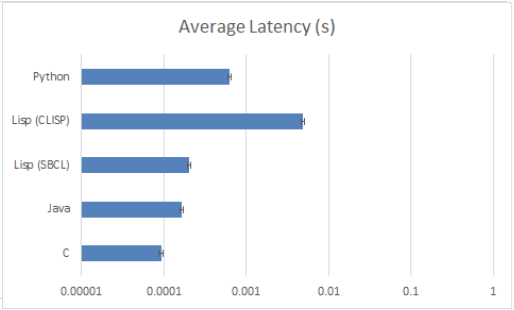
\includegraphics[width = 0.5\textwidth]{latency.PNG}}
\caption{Latency for encrypting or decrypting a 1417 byte message.}
\label{fig:lan}
\end{figure}

In figure \ref{fig:lan} we see that the fastest language by far is C with just under 100 milliseconds. Closely following is Java and the SBCL Lisp result. The Python and GNU Clisp results are the slowest. Especially the GNU lisp with a latency almost approaching one hundreth of a second.

\begin{figure}
\centerline{ 
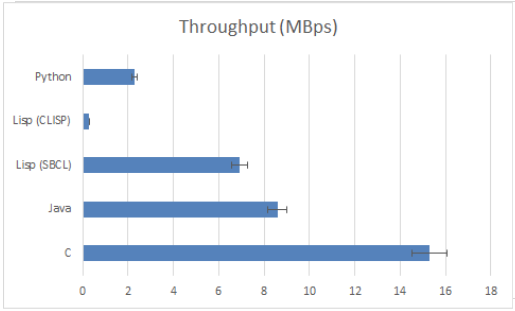
\includegraphics[width = 0.5\textwidth]{throughput.PNG}}
\caption{Throughput for encrypting or decrypting bytes.}
\label{fig:ban}
\end{figure}

Similar trends are shown in the throughput. With C being the leader, followed in the same order by Java, SBCL, Python, and GNU Clisp. Overall it is not surprising that C wins in terms of performance. With Lisp one must be careful with what interpreter/compiler is used. Java possesses decent performance and Python is slow.

\subsection{Qualitative Analysis}

No language, even Cryptol, adequately protects against timing attacks as each will allow a programmer to utilize the length of a secret 
to define the number of iterations in a recursive statement or a loop. This is a difficult issue as it would require the programmer to 
either classify a piece of data as a secret, perhaps similarly to how a variable can be \texttt{const} or \texttt{static} in C.

While Cryptol allows for us to easily verify the correctness of a program it is not clear how to use or even benchmark the verified program 
in an easy to use manner. Ideally one would be able to compile the verified implementation to a binary for use in other programs as a linkable 
library or package. This would allow the average programmer to more reliably and verifiably implement a cryptographic algorithm or cipher.
